\subsection{Le calorimètre électromagnétique ou ECAL}\label{chapter-LHC-section-CMS-subsec-ECAL}
%\cite{cms_paper,CERN-LHCC-97-033,CMS-CR-1999-006,CMS-EGM-11-001,CMS-CR-2014-410,CMS-DP-2016-031,CMS-CR-2018-162,CMS-DP-2019-005,CMS-DP-2020-021}
Le calorimètre électromagnétique (ECAL)~\cite{cms_paper,CERN-LHCC-97-033,CMS-EGM-11-001,CMS-DP-2019-005,CMS-DP-2020-021} permet de mesurer l'énergie des électrons et des photons par un processus destructif.
Le ECAL est composé d'environ \num{76000} cristaux de tungstate de plomb (\ce{PbWO4}) dans lesquels les électrons et les photons forment une gerbe électromagnétique dont l'intensité du signal lumineux permet d'en obtenir l'énergie.
\begin{figure}[h]
\centering
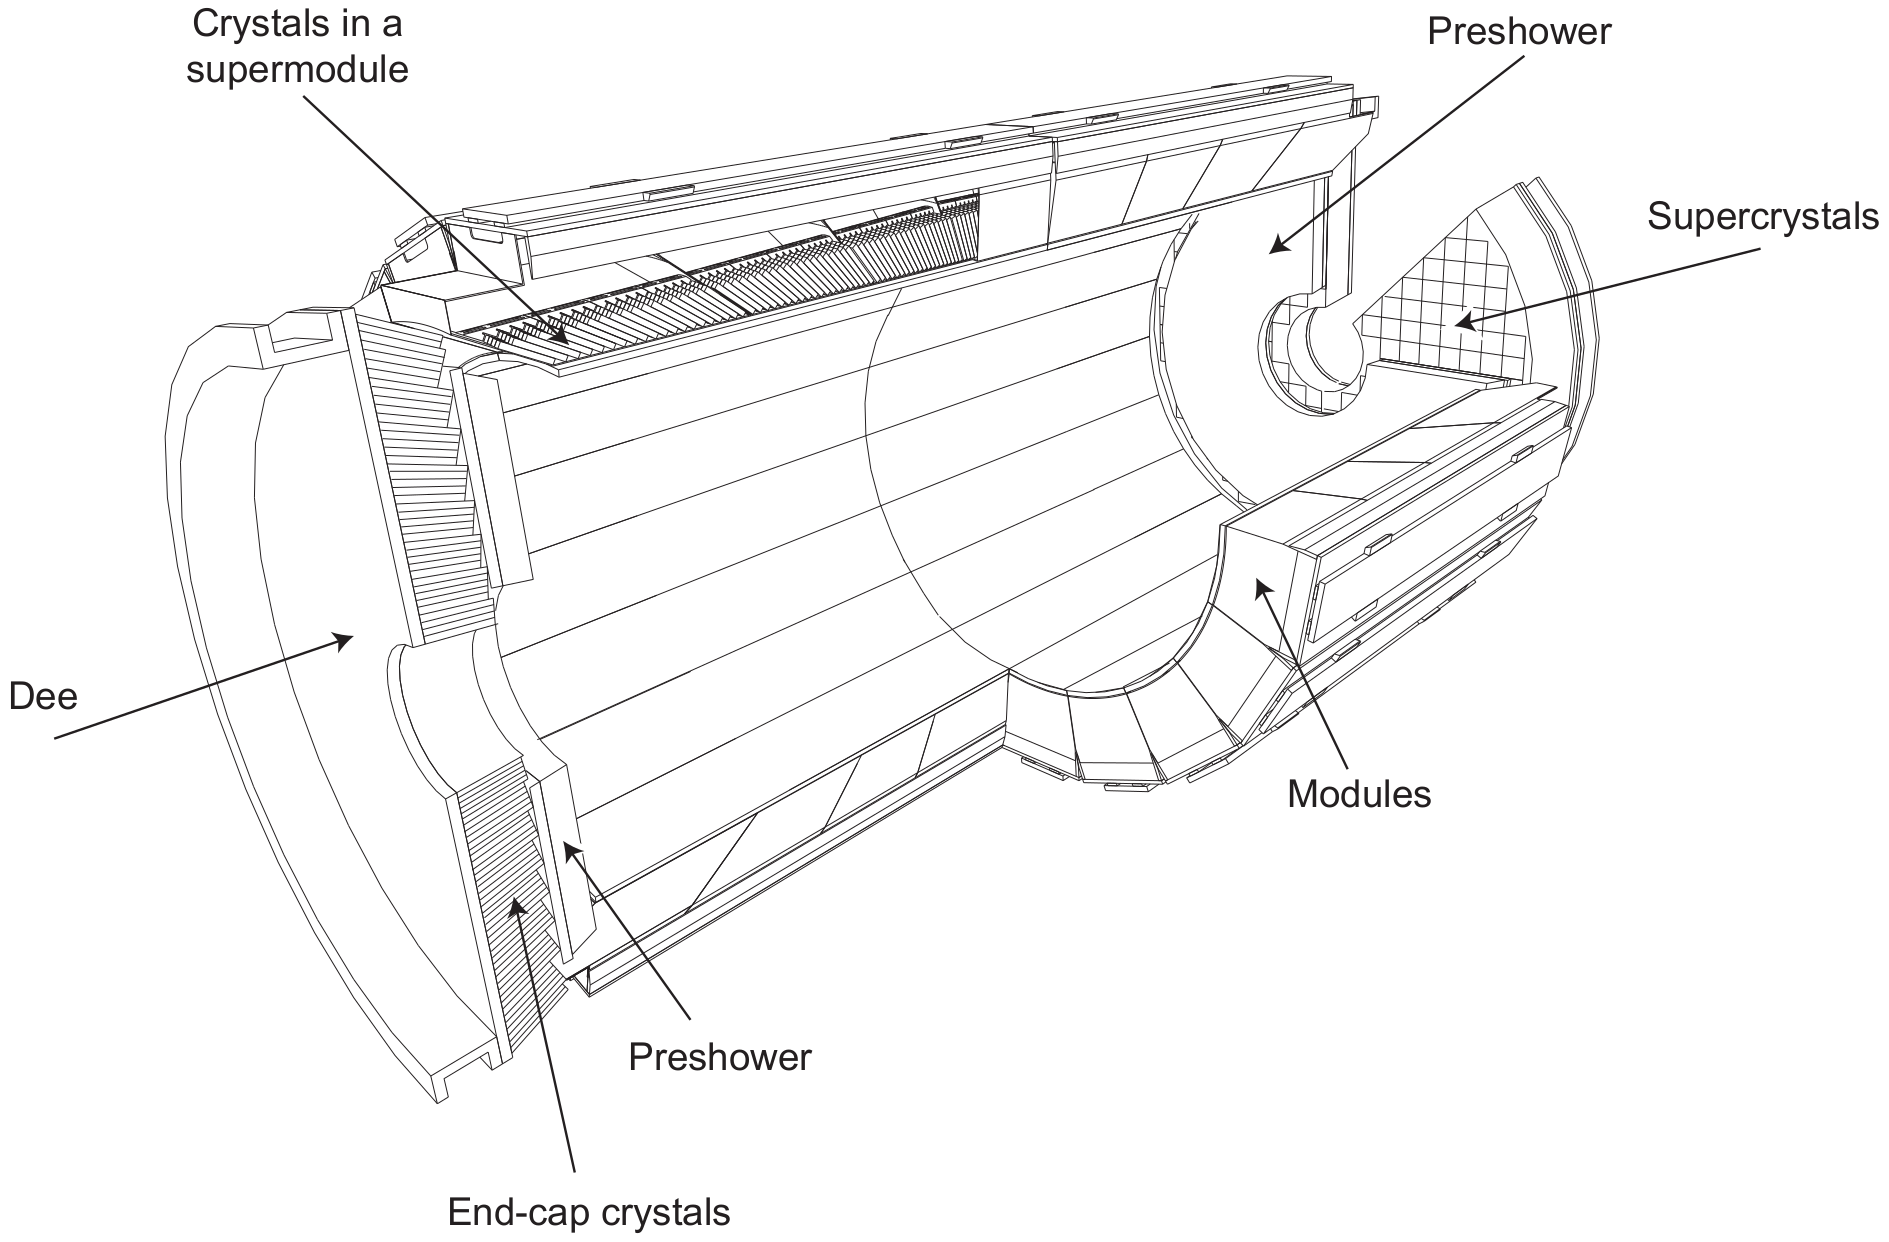
\includegraphics[width=0.8\textwidth]{\PhDthesisdir/plots_and_images/from_CMS-EGM-11-001/figures_calorimeter.png}
\caption[Schéma du calorimètre électronique de CMS.]{Schéma du calorimètre électronique de CMS~\cite{cms_paper,CMS-EGM-11-001} montrant le positionnement des cristaux, modules et supermodules dans le barillet, des supercristaux et du détecteur de gerbes dans les bouchons.}
\label{fig-chapter-LHC-section-CMS-subsec-ECAL-CMS-EGM-11-001-figures_calorimeter}
\end{figure}
\par Le ECAL se divise en trois sous-parties, schématisées sur la figure~\ref{fig-chapter-LHC-section-CMS-subsec-ECAL-CMS-EGM-11-001-figures_calorimeter}.
La première, comme pour le trajectographe, constitue la partie barillet du ECAL (EB) et couvre la région $\abs{\eta}<\num{1.479}$.
Le front des cristaux du EB se trouvent à \SI{1.29}{\meter} du faisceau.
Ils sont regroupés en \og modules \fg{} de \num{400} à \num{500} cristaux et quatre de ces modules forment un \og supermodule \fg{} de \num{1700} cristaux.
Le tour complet du barillet comporte \num{18} supermodules, chacun couvrant \ang{20} en $\phi$ et la moitié de l'espace en $\eta$ du EB.
Le EB complet est ainsi formé de \num{36} supermodules.
\par Les deux autres parties du ECAL forment les bouchons, couvrant la région $\num{1.479}<\abs{\eta}<\num{3.0}$.
Les bouchons du ECAL (EB) se trouvent à \SI{315.4}{\centi\meter}\footnote{Cette distance prend en compte le mouvement de \SI{1.6}{\centi\meter} de cette partie du détecteur lorsque le champ magnétique de \SI{3.8}{\tesla} est présent.} du point de collision le long de l'axe du faisceau.
Sur deux demi-disques (\emph{dee}) par bouchon sont répartis des \og supercristaux \fg{} formés de $5\times5$ cristaux.
\par Devant les EB se trouvent les détecteurs de gerbes (PS, \emph{PreShower}).
Leur rôle est d'identifier les pions neutres\footnote{Les pions neutres se propagent sur des distances moyennes de \SI{26}{\nano\meter} puis se désintègrent dans \SI{99}{\%} des cas en deux photons~\cite{PDG_booklet_2018}. Ce sont donc ces deux photons que le PS doit identifier.} dans la région $\num{1.653}<\abs{\eta}<\num{2.6}$.
Ils aident également à discriminer les électrons vis-à-vis des particules ionisantes ainsi qu'à la détermination des positions des photons et électrons.
Le PS est composé d'une couche de plomb initiant la gerbe électromagnétique suivie d'un détecteur à fils de silicium mesurant les dépôts d'énergie.
\par Le tungstate de plomb est très dense, \SI{8.29}{\gram.\centi\meter^{-3}}, et transparent.
Ce matériau possède également une faible longueur de radiation, $X_0=\SI{0.89}{\centi\meter}$, ainsi qu'un rayon de Molière de \SI{2.19}{\centi\meter}.
Le ECAL présente une réponse rapide, une bonne granularité et une résistance suffisante aux radiations.
Près de \SI{80}{\%} du signal lumineux émis dans les cristaux du ECAL par les électrons et photons se trouve en effet dans une fenêtre temporelle de \SI{25}{\nano\second}, la durée entre deux événements successifs au LHC~\cite{cms_paper}.
Dans le cas des hadrons, la traversée des cristaux du ECAL correspond approximativement à une longueur de radiation.
Près des deux tiers des hadrons commencent ainsi une gerbe électromagnétique avant d'arriver dans le calorimètre hadronique, sous-détecteur suivant.
\par La longueur des cristaux, \SI{23}{\centi\meter} dans le barillet et \num{22} dans les bouchons, correspond à \num{25.8} longueurs de radiation dans le barillet et \num{24.7} dans les bouchons, permettant de d'absorber \SI{98}{\%} de l'énergie des électrons et photons jusqu'à \SI{1}{\TeV}.
Ces particules ne se propagent donc pas, en bonne approximation, dans les parties suivantes du détecteur.
\par La réponse des cristaux du ECAL est contrôlée régulièrement à l'aide de laser afin d'évaluer leur réponse~\cite{CMS-DP-2019-005}.
La figure~\ref{fig-chapter-LHC-section-CMS-subsec-ECAL-CMS-DP-2019-005-histories_2011-2012-2015-2016-2017-2018_190208} présente l'évolution de la réponse des cristaux du ECAL depuis le début de l'exploitation du LHC.
La réponse se dégrade au cours du temps car les cristaux, bien que peu sensibles aux radiations, se trouvent dans un environnement à très fortes radiations.
Une perte de la transparence des cristaux est ainsi inévitable, diminuant leur réponse.
Des corrections sont alors appliquées afin d'assurer une stabilité temporelle de la réponse du ECAL.
De plus, la réponse des cristaux présente une forte dépendance thermique, de l'ordre de \SI{2}{\%.\degC^{-1}}.
Un système de refroidissement assure une stabilité de la température des cristaux à $\pm\SI{0.5}{\degC}$.
\begin{figure}[h]
\centering
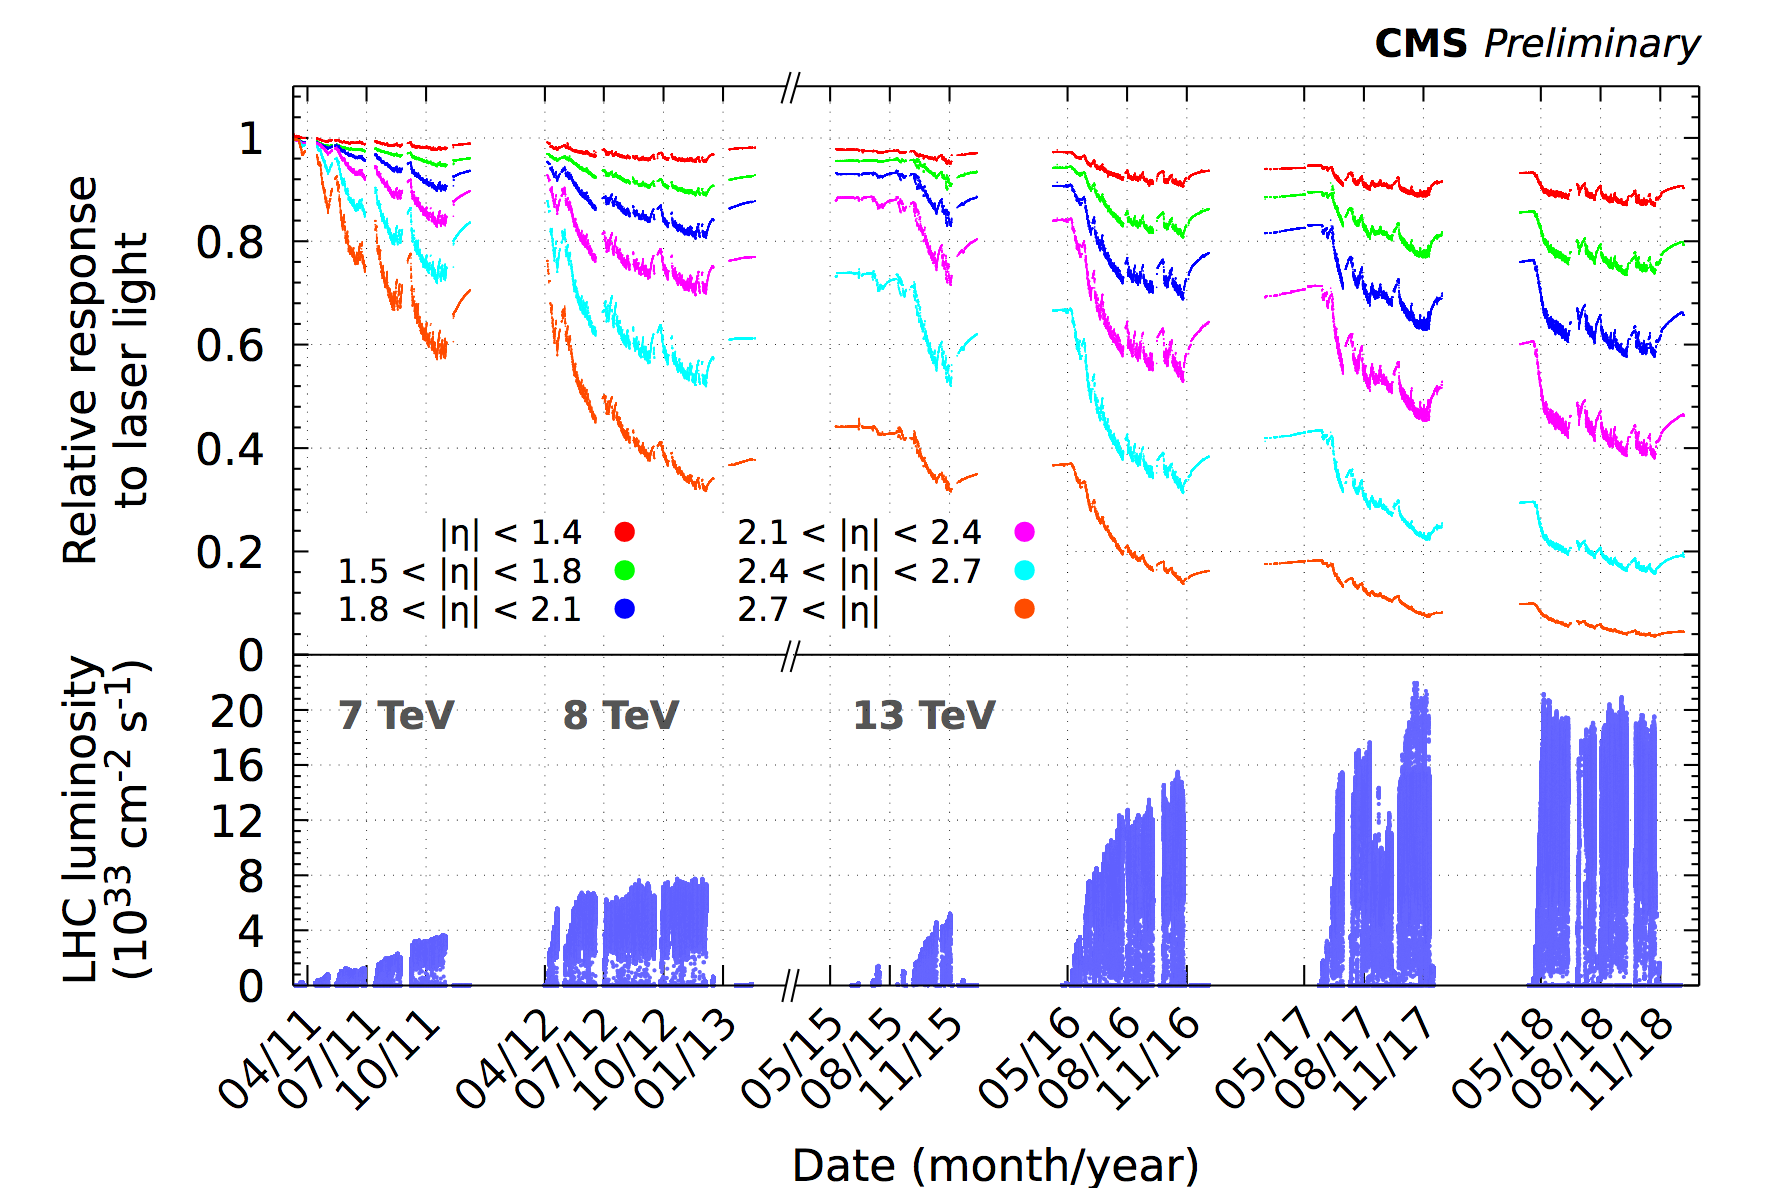
\includegraphics[width=.75\textwidth]{\PhDthesisdir/plots_and_images/from_CMS-DP-2019-005/histories_2011-2012-2015-2016-2017-2018_190208.png}
\caption[Évolution temporelle de la réponse du ECAL.]{Évolution temporelle de la réponse du ECAL~\cite{CMS-DP-2019-005} (haut) et luminosité instantanée du LHC (bas).}
\label{fig-chapter-LHC-section-CMS-subsec-ECAL-CMS-DP-2019-005-histories_2011-2012-2015-2016-2017-2018_190208}
\end{figure}
\par La résolution $\sigma$ du ECAL est paramétrée selon
\begin{equation}
\frac{\sigma}{E}
=
\frac{S}{\sqrt{E}}
\oplus
\frac{N}{E}
\oplus
C
\end{equation}
où $\oplus$ désigne une somme quadratique, \ie\ $(a\oplus b)^2 = a^2 + b^2$,
$S$ un terme stochastique prenant en compte la largeur latérale de la gerbe électronique,
$N$ le terme de bruit des composants électroniques et
$C$ une constante rendant compte des erreurs de calibration.
Des tests en faisceau réalisés en 2006~\cite{cms_paper} ont permis de mesurer
$S = \SI{0.028}{\GeV^{1/2}}$,
$N = \SI{0.12}{\GeV}$ et
$C = \num{3.0e-3}$.
La figure~\ref{fig-chapter-LHC-section-CMS-subsec-ECAL-CMS-DP-2020-021-final_Resolution_RunII_Inclusive} présente ainsi la résolution relative du ECAL sur l'énergie des électrons lors du Run~II.
\begin{figure}[h]
\centering
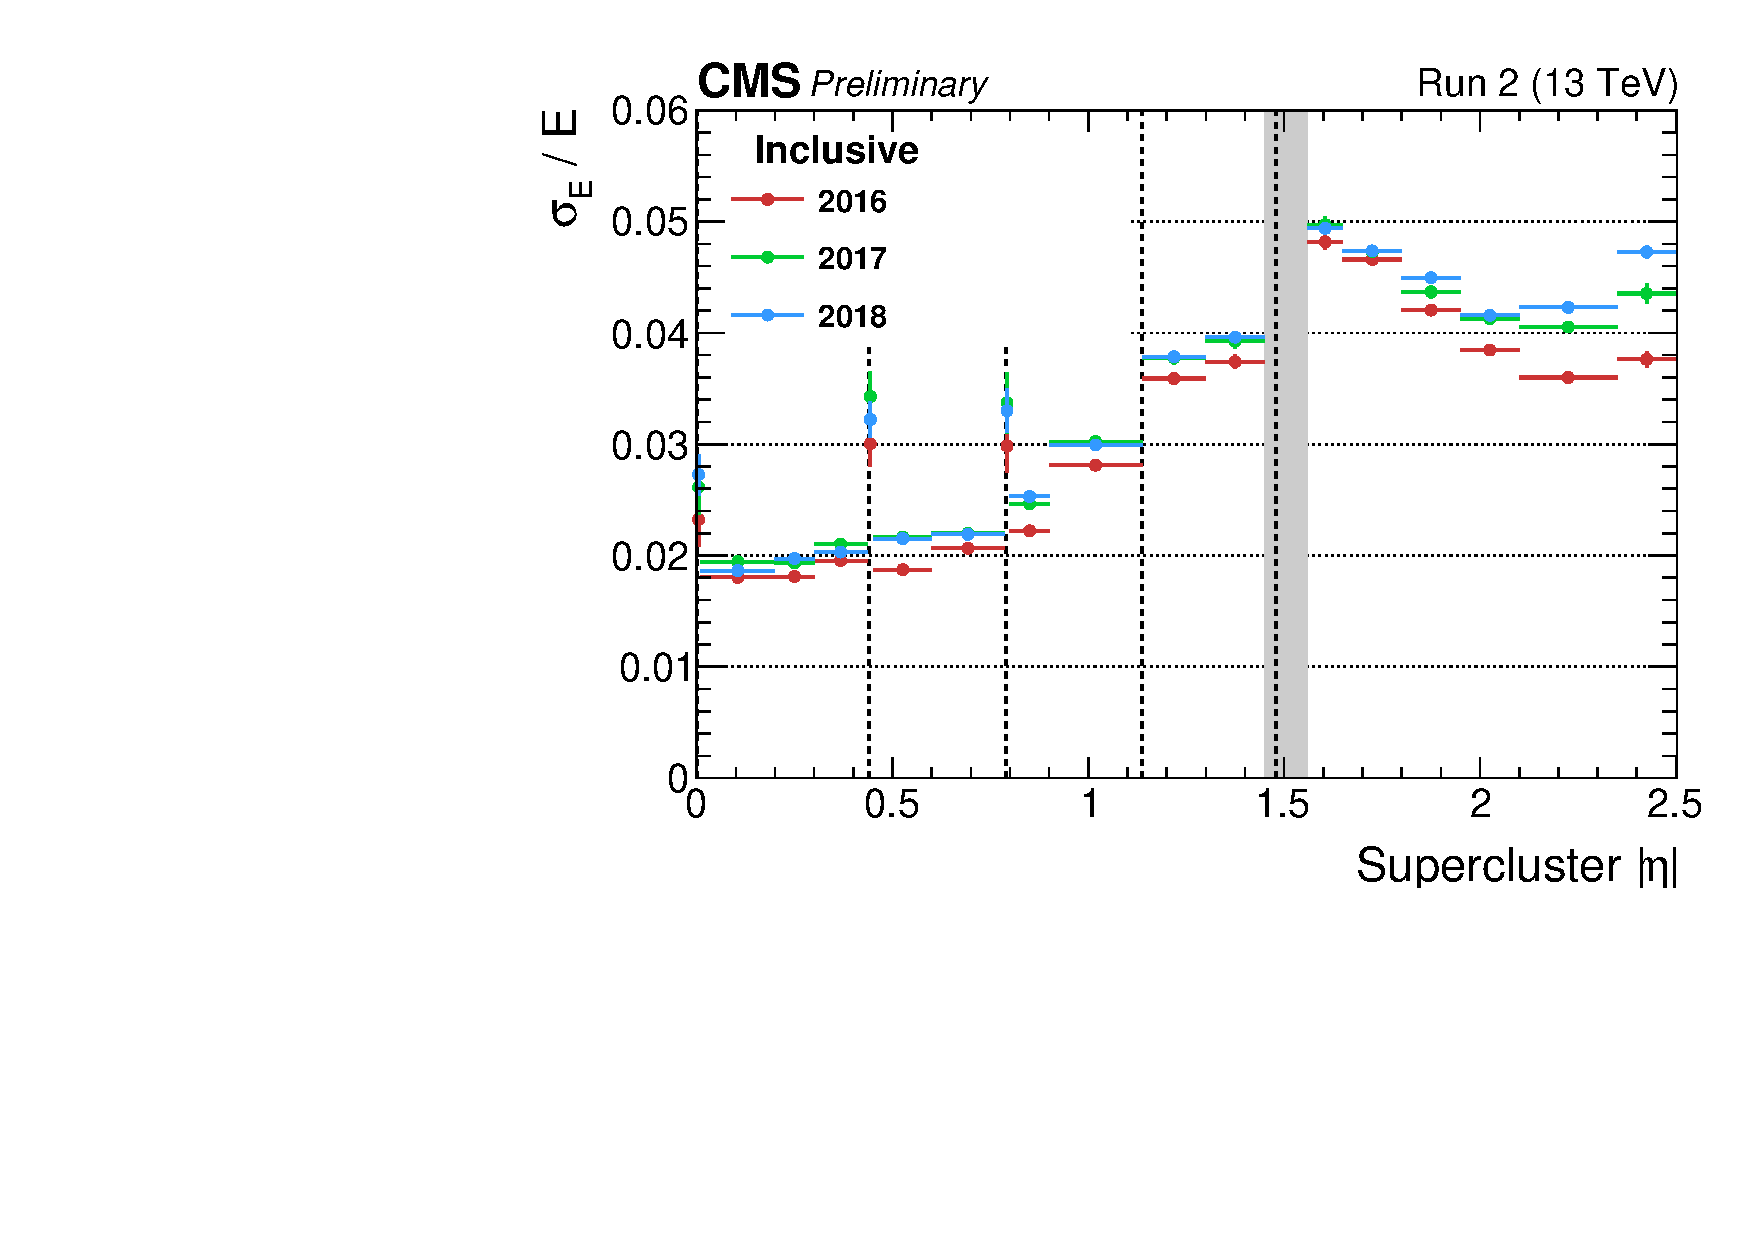
\includegraphics[width=.55\textwidth]{\PhDthesisdir/plots_and_images/from_CMS-DP-2020-021/final_Resolution_RunII_Inclusive.pdf}
\caption[Résolution relative de l'énergie des électrons dans le ECAL lors du Run~II.]{Résolution relative de l'énergie des électrons dans le ECAL lors du Run~II en fonction de $\eta$~\cite{CMS-DP-2020-021}. La résolution est obtenue à partir d'événements $\Zboson\to\antielectron\electron$.}
\label{fig-chapter-LHC-section-CMS-subsec-ECAL-CMS-DP-2020-021-final_Resolution_RunII_Inclusive}
\end{figure}